%\part{Background}
\chapter{Recommender Systems}
\label{chap: Chapter 2}

The focus of this chapter is to identify a research problem and methodology which needs to be followed.

In this chapter, we discuss the background and related work of recommender systems. The following section discusses the history of information retrieval and how it ties in with information filtering. After that, the various methods of recommender systems will be addressed. In the latter sections, a high-level overview will be discussed of the components in a recommender system. The chapter concludes with state-of-the art recommender systems.

\section{Information Retrieval}

We live in an information age surrounded by technology. Information is the lifeblood of the technological ecosystem that is spread using smartphones, tablets, and other computing devices. Owing to technological advances, information is easily created or distributed. It is apparent that with the ever-increasing creation of information, researchers are experiencing information overload, which has a direct influence on academic performance \cite{binti2017influence}.

Information overload can be defined as when an individual, who needs to make a decision, is trying to ingest a large amount of data, and the amount of data is larger than the individual’s capacity to process the information \cite{Heylighen2002ComplexityAI}.
Researchers have learned to combat information overload by employing tools consisting of new technology to expose only the information that is relevant to them, known as information filtering \cite{Hanani2001}. 

Information filtering systems stretch across multiple domains and are useful for extracting information out of unstructured or semi-structured information bodies like e-mails and documents, for large amounts of text, and lastly, it can also keep account of  the activities of various user profiles.

The above features are not only limited to information filtering systems but also information retrieval. It is important to remember that information filtering and information retrieval do work similarly, but differ in characteristics indicated below, and in summary in Table \ref{tab:DIFCBFIR}.

\begin{enumerate}
    \item Frequency of use – information retrieval [IR] systems are designed for one-time, ad hoc users, whereas information filtering [IF] systems are created for repetitive uses.
    \item Representation of information needs – in information retrieval systems, users interact with queries. In contrast, in information filtering systems, the long-term needs of users are best saved in user profiles.
    \item Goal – information retrieval systems select the information stated in the query out of the database. Information filtering systems just filter out irrelevant data.
    \item Database – information retrieval systems usually employ static databases to store and retrieve information. Information filtering works with dynamic data.
    \item Types of users – information retrieval systems do not know the users, and anyone can pose a query. Users of information filtering systems need to be known, since the system has models of all the user profiles.
    \item Index – information retrieval systems index data based on items and information filtering systems index based on user profiles.
\end{enumerate}

\begin{table}[]
\centering
\resizebox{\textwidth}{!}{%
\begin{tabular}{|l|l|l|}
\hline
\textbf{Characteristics}     & \textbf{Information Retrieval}                                                                                                    & \textbf{Information Filtering}                                                                                                                                   \\ \hline
Frequency of use             & ad-hoc use                                                                     & \begin{tabular}[c]{@{}l@{}}long term users \end{tabular}                                                     \\ \hline
Representation of information needs & queries                                                                                                        & user profiles                                                                                                                                  \\ \hline
Goal                         & \begin{tabular}[c]{@{}l@{}}selecting relevant items \end{tabular} & \begin{tabular}[c]{@{}l@{}}filtering out irrelevant data\end{tabular} \\ \hline
Database                     & static                                                                                                         & dynamic                                                                                                                                        \\ \hline
Type of users                & not known to the system                                                                                        & \begin{tabular}[c]{@{}l@{}}known to the system,\\ a user model\\ is saved in the system\end{tabular}                                           \\ \hline
Index              & items                                                                                        & \begin{tabular}[c]{@{}l@{}}user profiles\end{tabular}                                                        \\ \hline
\end{tabular}%
}
\caption{Comparison between IR and IF systems}
\label{tab:DIFCBFIR}
\end{table}

As highlighted in Table \ref{tab:DIFCBFIR}, information retrieval and information filtering does work similarly but there are some differences at their core. \citeA{resnick1997} mention that sources suggest using recommender systems to tailor content to users.

The aim of information filtering (IF) is to show only the items that are relevant to the users \cite{Hanani2001}. The idea was that Information Filtering can be more effective when humans are involved in the filtering process \cite{Hanani2001}.

Because the spike of product information makes it harder for users to find what they are looking for online, e-commerce sites like Amazon.com use collaborative filtering based on purchase history and customer ratings to make personalised recommendations.

Since the introduction of collaborative filtering in the 1990s, recommender systems have grown to be a very important research area \cite{resnick1994grouplens,shardanand1995social}. The term ‘collaborative filtering’ was coined in 1992 by Goldberg when implementing one of the first spam-filtering systems \cite{goldberg1992using}.

‘A recommender system is defined as a tool that can recommend a list of items to a particular set of users based on the user’s preferences’ \cite[p.~4]{ricci2011introduction}.

They have successfully applied recommender systems to different domains such as e-commerce, movies, news, music, research, just to name a few. For example, on Amazon and Netflix users buy and watch more content that is recommended to them \cite{Andre2018} now that the gravity of recommender systems is emphasised.

\citeA{adomavicius2005toward} have identified three types of recommendation methods. They are:
\begin{enumerate}
    \item Collaborative filtering (CF)
    \item Content-based filtering (CBF)
    \item A hybrid method
\end{enumerate}
In the following section, we will discuss the various types of recommendation methods.

\section{Collaborative Filtering (CF)}  \label{sec:collab}

Collaborative filtering systems assume that a user will like the same items as another user liked in the past. Collaborative filtering systems are popular and are commonly used in online shopping websites \cite{Nilashi20161}.

Collaborative filtering focuses recommendations based on similarities between user ratings. Content-based filtering works a bit differently from collaborative filtering, in that users get recommendations based on other users’ preferences in the past. Lastly, the hybrid recommender system employs both collaborative filtering and content-based filtering methods.

In recent years, researchers adapted the traditional content-based filtering approach to move towards preference-based filtering. This subdomain focused on predicting items based on the users’ preferences \cite{william1999learning,freund2003efficient,jin2002preference,jin2003collaborative}. For example, preference-based filtering can predict movies based on their order relative to each other and not on individual ratings. As stated in the delineation of this dissertation, the focus will be on rating like-based recommendations since it is a popular approach \cite{park2012literature}.

The collaborative filtering (CF) approach works by predicting user preferences for items through learning from past user-item relationships \cite{celma2008new}. Users give feedback to the system through their preferences or ratings and then the recommender system provides a list based on the feedback.

One of the first recommender systems that used the collaborative filtering method was Ringo, a music recommender system \cite{shardanand1995social}. A few other systems that have employed collaborative filtering in that time period can be found in \citeA{resnick1994grouplens}.

Each method has several advantages and disadvantages, which would guide recommender system implementation to fit the use case.
An argument in favour of using collaborative filtering is that implementing Memory based filtering is easy \cite{Girase}. For example, memory-based methods use historic rating data between users or items to recommend items to people. Another positive aspect is that memory-based filtering would be preferred when new data is continuously supplied to the model \cite{jannach2010recommender}. Full updates can be made  continuously to the recommending system.

In contrast to the advantages of collaborative filtering, it also does have disadvantages. Some occur when collaborative filtering runs into a general issue called the cold start problem. That is when a new user is introduced to the system, and the system does not know what to recommend to the user.

Collaborative filtering is also less scalable since some systems generate recommendations for billions of user-item pairs. Finally, in some cases, collaborative filtering systems have been found to be manipulated by users promoting their own items \cite{resnick1994grouplens}.

Collaborative filtering is classified into two methods: memory-based- and model-based collaborative filtering \cite{naak2009multi}.

\subsection{Model based collaborative filtering} 

This creates and builds an offline statistical model based on the user-item pairs seen in the training set. Once the model has been built, it is then applied in an online setting to recommend as intended \cite{jannach2010recommender}. Several techniques are being used in model-based collaborative filtering, such as probabilistic techniques \cite{pavlov2004collaborative}, and graph- based techniques \cite{clements2009exploiting}.

The preferred ones are the latent factor models that reduces the dimensionality of the matrix and uncover latent topics between users and items. Some examples of latent factor models include: singular value decomposition (SVD) for matrix factorisation \cite{clements2009exploiting} and probabilistic latent semantic analysis (pLSA).


\subsection{Memory based collaborative filtering}
\citeA{jannach2010recommender} describe memory-based collaborative filtering as recommendations that are being made on the entire user-item rating matrix. It computes distance or correlation measures to find user/item similarities. Furthermore, memory-based collaborative filtering looks for either neighboured users for the target user, user-based, or pairs of items that are rated by other users (item-based).

In the next section, the content-based filtering method will be discussed, followed by its advantages and disadvantages.

\section{Content-based Filtering} \label{sec:content}
The content-based approach to recommendation has its roots in the information retrieval (IR) and information filtering (IF) research field. Recently, much research has been undertaken in the recommendation systems, information retrieval and information filtering fields.

Pushing the boundries in terms of what each field can do, content-based filtering methods analyse a set of features of items that are relevant to the user and link the user profile based on those items. In essence, the method links the users to the items \cite{lops2011content}.

There are a few comparisons that can be made between content-based filtering and IR, outlining the differences and similarities \cite{belkin1992information}. The common goal between content-based filtering and IR systems is to select items that are relevant to the users.

For example, suppose the user is looking for a similar or set of similar research papers. In that case, the content-based recommender system will recommend research papers based on the themes found in the current paper; thus, leading us to the advantages and disadvantages of content-based recommender systems.

One of the disadvantages found in collaborative filtering, is a strength in content-based filtering. In contrast to collaborative filtering, the cold-start problem does not apply to content-based filtering since the recommendations are not made based on ratings from other users.

In addition to the non-existent cold-start problem, building a content-based filtering recommender system is straightforward and significant in terms of  adding incremental data to the models.

On the other hand, content-based filtering does have difficulty in generating the features of the items. There are limits to the number and types of features that one can generate from items.

In addition to the features, domain knowledge is needed. For example, for research paper recommendations, the system needs to have quite a lot of data regarding each document, including data such as what topics are being discussed, and which branch in that specific topic are being covered. The system needs to distinguish between what the user likes and what not \cite{lops2011content}.

Content-based filtering often suffers from over-specialisation since it recommends the same types of item. For example, when inputting a ransomware research paper into the recommender system, it will only show research papers which also contain ransomware-related topics. This issue is called serendipity. Content-based recommender systems tend to lack novelty awareness \cite{shah2018}.

In the next section, the high-level architecture of a recommender system will be discussed.

\section{High level Architecture of Recommender Systems}

\begin{figure}[htbp]
\centering
\includegraphics[width=10cm]{./figures/overviewRS1.png}
\caption{Overview of Recommender Systems}
\label{fig:OverviewRS}
\end{figure}

This section focuses on introducing the high-level architecture of a recommender system. Each component will be discussed in relation to collaborative filtering and content-based filtering methods.

As seen in Figure \ref{fig:OverviewRS}, in both recommender system methods, we see similar components. One component is that of similarity, either between articles or between other users. Both of the methods have a learning component where machine learning or information retrieval methods can be employed.

More components will be introduced later in this section. Recommender systems are strung together to attain a certain goal. The high-level architecture, portrayed in Figure \ref{fig:archRS}, will be discussed now:

\begin{figure}[htbp]
\centering
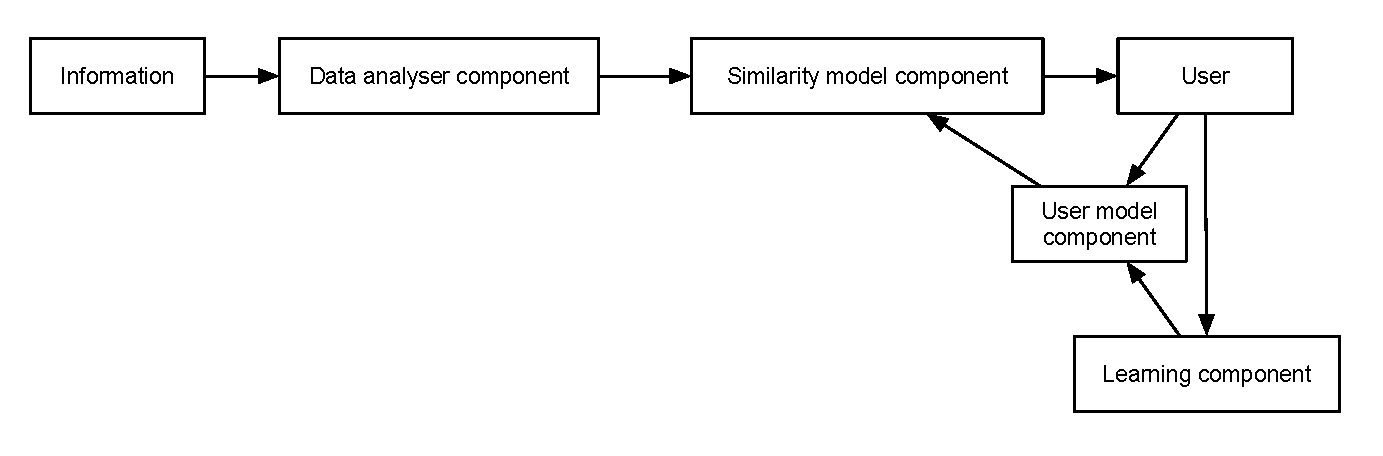
\includegraphics[width=12cm]{./figures/arch12.eps}
\caption{Architecture of Recommender Systems}
\label{fig:archRS}
\end{figure}

\begin{itemize}
    \item The data analyser component – the items are obtained or collected (e.g. documents) from information providers. The items are then analysed and represented in a readable format (e.g. in a vector of index terms).
    Such a vector will be the input to the similarity model component.
    \item The user/item model component – it gathers information about the user and their needs (explicitly and/or implicitly) and is constructed as user profiles. Then the user profiles will also serve as input to the similarity filtering component. In most collaborative filtering recommender systems, users will have items recommended based on their item model.
    When the system recommends items, it will compare similar users.
    \item The similarity model component – it consists of matching the user profile or item models to the corresponding items and calculating the similarity between them.
    \item The learning component – the user who gets the relevant data item is ultimately the catalyst for feedback. Furthermore, the data is then updated with the new user preference to improve further predictions.
\end{itemize}

Various methods and techniques can be used to integrate content-based recommender systems: There are many ways to analyse data items and to represent them in better ways, ultimately to gain more knowledge from the user to implement back into  the user models. More of those techniques will be discussed in Chapter \ref{chap: Chapter 3}.

Content-based filtering methods can be divided into two categories: (1) models built in machine learning, such as neural networks, naive Bayes model and decision trees \cite{lops2011content}, or (2) heuristic functions stemming from information retrieval techniques \cite{cantador2010content,diederich2006finding}. The machine learning (ML) methods try to classify new items that are relevant or not for each user. The authors \cite{lops2011content} used the naive Bayes model to create a probabilistic model to recommend items to users.

The naive Bayes model calculates the probability whether the item is relevant or not. However, most content-based filtering methods are based on a heuristic approach, which represents users and items are vectors of TF-IDF \cite{jones2004statistical} or BM25 \cite{baeza1999modern} in a vector space model (VSM).

VSM is a spacial representation of the text documents where each document is represented by a vector in an n-dimensional space. Each dimension corresponds to a term from the overall vocabulary of a document. Recently, the most popular term-weighting scheme is TF-IDF that considers terms occuring frequently in one document, but do not occur as much in the rest of the corpus.

Now to compare the two filtering methods, collaborative filtering and content-based filtering, content-based filtering allows for user independence, which means that it does not use the other user ratings to find the nearest neighbours. Content-based filtering uses the ratings provided by the targeted user to build their own profile. However, one of the most common limitations that occurs in content-based filtering methods is that the content-based filtering methods cannot provide recommendations if the content does not have enough features to distinguish one from another \cite{lops2011content}.

Furthermore, this phenomenon raises the need to create domain knowledge to link new features to new items. For instance, commonly in a movie recommendation system one of the components is to use an external source, like an ontology, to know who the actors and directors are of the movie. Another limitation of using content-based filtering is that it recommends exactly the same content as that which the user already rated. This is called the serendipity problem \cite{DEGEMMIS2015695}. Also, content-based filtering methods cannot recommend items before they have gathered enough data from the user, and this is called the cold-start problem \cite{LIKA20142065}.


\section{Hybrid Method}
The term hybrid recommender system comes from the combination of collaborative- and content-based filtering techniques. The combination of the two increases their individual performances by reducing the severity of the cold-start problem. On the other hand, it will diversify the recommendations given to the user. Three base designs of hybrid recommender systems were presented by \citeA{burke2002hybrid}. These are:

\begin{enumerate}
    \item One base design is a single recommender system that considers a wide range of input data from other recommendation techniques in one algorithm implementation \cite{dong2017hybrid}. For example, a hybrid system was proposed to combine features like user ratings, and features of the items.
    \item Furthermore, another design made an appearance by combining the two methods. The combination was not in series, but rather parallelised \cite{sharma2016evolution}, taking each method’s output and recommending both to the user.
    \item Lastly, recommender systems are joined together in a pipeline where the output of one recommender system is the input of the other one.
\end{enumerate}

\section{Summary}
The rise of information creation and content on the internet has created a problem. In the problem, it was found that researchers are experiencing cognitive barriers. These barriers include not knowing which pieces of information are relevant to their study, and actually not obtaining the correct information to include in their studies.

Information filtering and information retrieval were discovered, which aided the larger audience to scope down information to only a few lines. Many employed these techniques in various sections in the industry. These advances led to the creation of recommender systems.

Each type of recommender system has specific capabilities. This chapter gave a brief overview of what each recommender system method can achieve.  The chapter presented an architectural overview in Section \ref{fig:archRS}. The implementation of the recommender system relies on the use case of the implementer. 

For the use case in this study, the recommender system would need to have a level of insight with regards to the content.  This is necessary as the system would need to identify specific terminology of a given domain; in this case Information Security.  This study does not have access to historic recommendation data, but bases its insights on Information Security-related papers. 

As described in Section \ref{sec:collab}, collaborative filtering uses item and user pairing to recommend items that other users have liked in the past. Furthermore, collaborative filtering does not look at the content of items. The utility of collaborative filtering did not compliment the use case of the study, and therefore a content based recommender system was used.

The next chapter, Chapter \ref{chap: Chapter 3}, discusses the various technological concepts like machine learning, topic modeling, document clustering, and natural language processing.



